\chapter{Blockchain: A Practical Overview and Use Cases}\label{blockchain}

\begin{quote} 
  \emph{It was for a long time necessary, to establish trust between two
  entites, a middle-man with a netral stake. The blockchain aims to solve this
  depency using decentralization and a mechanism called consensus. A Blockchain
  is a distributed system which means that processing is shared across multiple
  nodes. Permissioned Blockchains are more suited towards enterprise and
  organizations while still benefiting from the immutability of the Blockchain
  architecture. Ethereum is a permissionless implementation whereas Fabric is
  Permissioned. Ethereum uses a currency to maintain the network while Fabric
  uses \textbf{BFT} consensus which does not need a currency. Both feature
  smart contracts even tough they feature different execution architectures.
  Ultimately, the Hyperledger Fabric Distributed Ledger Platform , with its
  focus on enterprise use and true data segregation, was chosen as the platform
  to build a system that seeks to achieve the purpose mentioned in
  Chapter~\ref{introduction}.}
\end{quote}

The Blockchain, initially used to solve problems in centralized financial
systems, has inherent characteristics that make it suitable for a variety of
use cases. This Chapter will provide a more practical exploration of the
Blockchain technology showing some of the considerations that were taken into
account, after analyzing some implementations of this technology, mentioned in
Chapter~\ref{background}.

\section{Trust in a Network}

Blockchain implementations are an emerging structure for distributed computing
systems that provide an immutable history of records written to a ledger, even
when there is no implicit trust relationship between the parties
involved~\cite{Barclay2017}.

Banks used to keep track of their financial transactions by writing on a book
usually located at the central bank. This book was often called ledger.
Whenever a transaction occurred someone wrote on the book. In short, the ledger
acts as a mean of storing all the transaction details between the bank and
other entities. 

Nowadays banks do not use the ledger in a book format. Instead the ledger is
referred to as the structure that holds all transaction information the bank
possesses. It is a structure that keeps the original purpose of recording all
the transactions that are made.

Imagine the following situation- Joe is on vacation and needs to borrow money
from Jane, his wife. Joe calls Jane to ask for some money and Jane tells him it
will send the money right away. Jane then proceeds to call her account manager
to transfer some of her money to Joe. Finally Jane calls Joe to tell him that
she made the request to send money to him.  As seen on
Figure~\ref{fig:centralizedvsdescentralized} Joe and Jane need to use and trust
the account manager and the bank as a middle man in order to complete this
transaction. If the bank was ever to be unavailable, the bank's database was
corrupted or if someone with  privileged access was able to intercept the
transactions from inside the bank then all transactions between Joe and Jane
would fail creating additional costs to all parties involved. 

\begin{figure}[h]
  \centering
  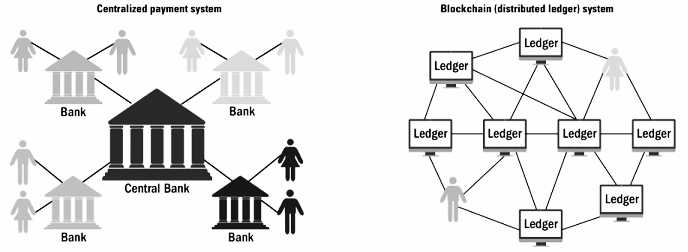
\includegraphics[width=1\linewidth]{imgs/blockchainvscentralizedNetwork.png}
  \caption{\label{fig:centralizedvsdescentralized} A comparison between a
  Centralized Banking System and a Distributed Ledger. (Source: Finance \&
  Development, 2016)}
\end{figure}

It was for a long time necessary, to establish trust between two entities, a
middle-man with a neutral stake. While the ledger is also at the core of the
Blockchain, this technology aims to solve the dependency placed upon third
parties using decentralization and aims to make two different entities trust
each other through constant replication of the ledger, a security mechanism
called consensus.  While consensus has a system performance impact due to the
necessary replication of data, it is a mechanism that establishes a set of
rules that defines if a sequence of transactions is considered valid.
Different Blockchain implementations often use a variety consensus protocols to
balance this trade-off.

\section{Permissionless and Permissioned Blockchain Implementations}


There are three types of computer systems, as seen on Figure
\ref{fig:typesofnetworks}. As previously mentioned in this Chapter, Blockchain
was created out of a desire to solve problems that are displayed in the
centralized financial systems that society is currently based upon.

\begin{figure}[h]
	\centering
	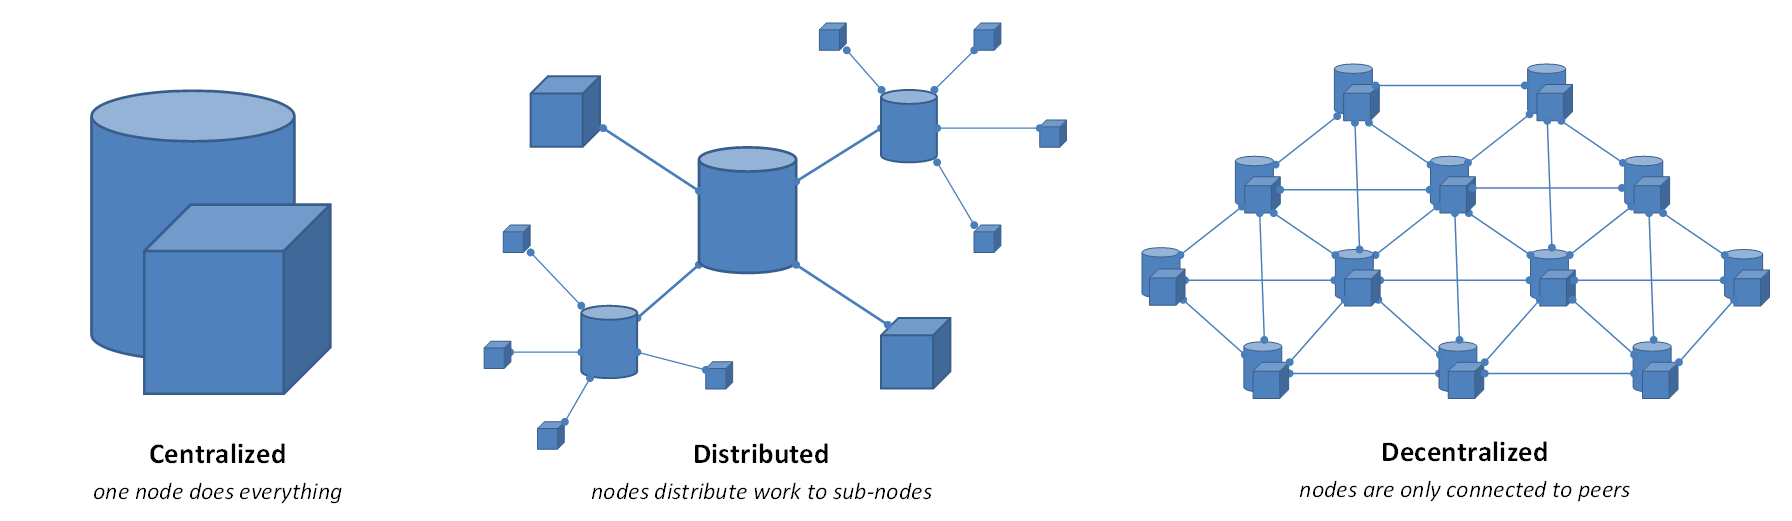
\includegraphics[width=1\linewidth]{imgs/typesofnetworks.png}
  \caption{\label{fig:typesofnetworks} A comparison between different types of
  systems. (Source: Eric Grange, 2016)}
\end{figure}

Put simply, a centralized system is one that is governed by a hierarchical
authority; examples of such being banks, credit card company’s, etc. If you
want to use a Visa card you must request access from Visa and be approved. At
any time your access to that line of credit and your funds may be made
unavailable to you and your access permanently revoked~\cite{Dreifuerst2018}.

In contrast, distributed systems are based upon the philosophy that processing
is shared across multiple nodes even if the decisions themselves may still be
centralized and use complete system state knowledge of the network. Finally, a
decentralized system is one where no single node can make a decision
individually, instead relying on the other participants to reach an agreement
and make a decision, as no single node has a complete system state knowledge.
With this in mind, a decentralized system is seen as a subset of a distributed
system.

A Blockchain is a distributed by design. However there are two major
implementation categories as discussed briefly on Chapter~\ref{background}.

Permisionless Blockchain implementations were the first to appear and while
some industries saw benefits in using the technology, some saw drawbacks to
adopting it in enterprise-grade systems~\cite{Gopinath2016} due to this
unregulated nature. They do have some advantages however compared to
traditional systems.

\textbf{Permisionless} Blockchain implementations, like the Bitcoin's and
Ethereum's Blockchain for example, have no barrier to entry. This means that
anyone can, in theory, participate in the network, write into it as a result of
mining and store data in the ledger sharing the work needed to maintain the
network.  Permisionless implementations have some strengths. These are
completely open and transactions are transparent while also being able to offer
anonymity or pseudo-anonymity. They also take away the need for system
administrators or central servers since the network is based exclusively on
peer-to-peer technology and decisions are made by every participant, creating
reduced costs to maintain and deploy \textbf{Ðapps}. On the other hand, these
implementations are slower than traditional systems because every node must
participate in consensus creating an overhead before a transaction is
considered verified. Due to this there is also a time cost associated because
of the need to wait until verification of the transaction. They operate without
clear legal rules and are trust-free, meaning that there is no responsible
entity if data loss or damages affect systems based on this implementation.

\textbf{Permissioned} Blockchain implementations have some clear advantages for
enterprise. They are faster because consensus is done by a set of nodes instead
of the entire network, can fall back on the legal system because it features an
identity service. This means the platform is auditable and that there is a
legal responsible entity or entities that manage the network. However, costs
when compared to the permissionless variant are higher due to having the need
for a system administrator and servers to manage the network, featuring a
private membership meaning that they are closed to the general public and
managed by a set of entities and are a compromise between the original vision
of a completely decentralized network and enterprise needs and concerns. 

Enterprises benefit greatly from the immutability of the Blockchain
architecture, in that all records cannot be changed. By adding authorized
identity services onto Blockchain, they can meet the regulatory needs of their
industries, by allowing the network to be auditable and assets to be traceable,
falling back to laws or regulations if a dispute between participating entities
occurs~\cite{Barclay2017}.

\section{A Decentralized Open Platform - Ethereum}

Ethereum is a permissionless Blockchain implementation. It is a platform that
lets anyone build and use decentralized applications commonly named
\textbf{Ðapps}. It is an open-source project developed primarily by the
Ethereum Foundation and was designed to be adaptable and flexible, in contrast
to Bitcoin's Blockchain that only records financial
transactions~\cite{EthereumDocs2018}.

It features a friendly programming language called Solidity that is influenced
by C++, Python and Javascript that is designed to allow an easy way for
developers to create new applications on the Ethereum platform with code of
arbitrary algorithmic complexity in a turing complete language. Smart Contract
application code targets the Ethereum Virtual Machine, which is then deployed
to the Blockchain via a local Ethereum node~\cite{Wood2017,Barclay2017}.

At the heart of Ethereum is the Ethereum Virtual Machine (\textbf{EVM}) as seen
on Figure~\ref{fig:evm} and, like any Blockchain, Ethereum also includes a
peer-to-peer network protocol. The Ethereum Blockchain database is maintained
and updated by many nodes connected to the network. Each and every node of the
network runs the \textbf{EVM} and executes the same instructions in order to
maintain consensus across the entire Blockchain. Decentralized consensus gives
Ethereum a high degree of fault tolerance, ensures zero downtime, and makes
data stored on the Blockchain forever unchangeable and
censorship-resistant~\cite{EthereumDocs2018}.

\begin{figure}[h]
  \centering
  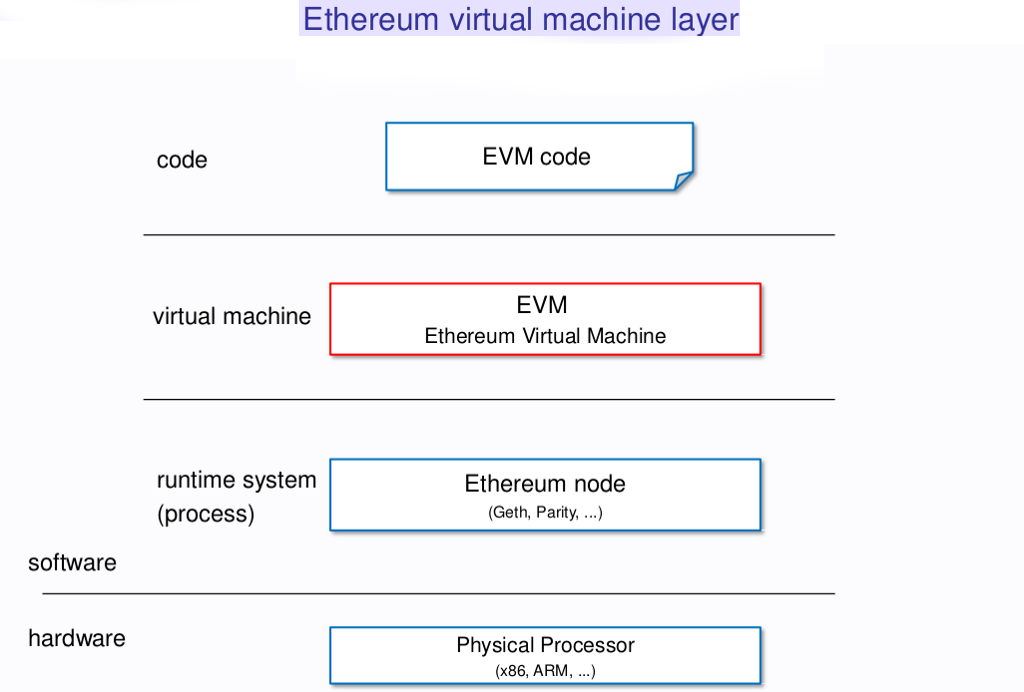
\includegraphics[width=1\linewidth]{imgs/ethereumVirtualMachine.png}
  \caption{\label{fig:evm} A diagram of where \textbf{EVM} fits into the
  Ethereum Platform (Original: Vaibhav Saini, 2018)}
\end{figure}

Users must pay a small transaction fee to the network each time they execute a
transaction. This protects the Ethereum Blockchain from frivolous or malicious
computational tasks, like Distributed Denial of Service (\textbf{DDOS}) attacks
or an infinite loop in smart contract logic. The sender of a transaction must
pay for each step of the “program” they activated, including computation and
memory storage. These fees are paid in amounts of Ethereum’s native
value-token, ether, and then these transaction fees are collected by the nodes
that validate the network commonly called miners - which are nodes in the
network that receive, propagate, verify, and execute transactions. Ethereum
currently uses a proof of work (\textbf{POW}) based consensus algorithm but
plans to change to a proof of stake (\textbf{POS}) algorithm due to
environmental and financial concerns as well as reduced centralization
risks~\cite{EthereumDocs2018,EthereumPOSFAQ2018}.

Ethereum has a live production network called “mainnet” available for any
developer to deploy applications to, as well as three test networks. "Ropsten”
is based on a \textbf{POW} algorithm while "Rinkeby" and "Kovan" are based on a
Proof of Authority~\footnote{In Proof of Authority based networks, transactions
and blocks are validated by approved accounts, known as validators. Validators
run software allowing them to put transactions in blocks. The process is
automated and does not require validators to be constantly monitoring their
computers. It does, however, require maintaining the authority node
uncompromised.} (\textbf{POA}) and all of them are publicly available and free
to use~\cite{Barclay2017,EthereumTestNetworks2018}.

Ethereum has had some unforeseen problems along the way, namely the
\textbf{DAO} heist where a hacker took advantage of a bug in a smart contract
to steal a great sum of money. With Ethereum frequently reaching full
transaction capacity, scaling solutions are the next big
investment~\cite{ethereumScalability2018}.

There are a few proposed solutions by Buterin. For example, \textbf{sharding}
is a solution that aims to avoid every node processing all data in order to
verify and process a transaction. When transactions are initiated they will not
be directed to all the nodes but would instead only be directed to those
depending on the shard in question.  Another solution is off chain computation
where a layer apart from the Blockchain is created and where all the
computation or solving of a complex mathematical equation takes place. This
would not only take the load off the Ethereum Blockchain but also help decrease
the cost of transaction verification and processing. This mechanism would
ensure that the tasks that account for slower transaction speeds on the
Ethereum’s Blockchain do not affect the whole network. Finally, to avoid every
node having the need to download the entirety of the Blockchain's data, the
complete picture can be stored on cloud and each node only has to store and
load relevant data~\cite{ethereumBlogScalability2018}.

\section{A Permissioned Distributed Ledger Platform - Hyperledger Fabric}
\label{distributedLedgerPlatform}

Hyperledger Fabric is a platform for distributed ledger solutions featuring a
modular architecture. It provides developers with a permissioned platform
targeted at business and enterprise use cases that supports pluggable
implementations of different components to accommodate the complexity and
intricacies that exist across the economic ecosystem. It is an open source
project initially commited by IBM  and estabilished under the Linux Foundation,
being developed by over 44 organizations and more than 250
members~\cite{HyperledgerFabricDocs2017,HyperledgerGrowth2018}.

It supports the creation of smart contracts, commonly called "chaincode" in
Fabric, that are authored in general-purpose programming languages such as
Java, Go and Node.js rather than constrained domain-specific languages
(\textbf{DSL}). 

Chaincode in Fabric consists of two components - the code itself, which
describes the logic of the program running in the execution phase, and the
endorsement policy that describes how a specific chaincode transaction is
validated. For example, a typical endorsement policy lets the chaincode specify
the endorsers for a transaction in the form of a set of peers that are
necessary for endorsement and subsequent successful
validation~\cite{Androulaki2018}. Chaincode runs in a container isolated from
the peer process which consented its installation providing aditional control
over information dissemination.

At the heart of Fabric is the permissioned distributed ledger that provides a
way to secure the interactions among a group of entities that have a common
goal but which may not fully trust each other. By relying on the identities of
the participants, a permissioned ledger platform can use a more traditional
crash fault tolerant (\textbf{CFT}) or byzantine fault tolerant (\textbf{BFT})
consensus protocols that do not require mining or an associated currency in
order to achieve consensus.

\begin{figure}[h]
  \centering
  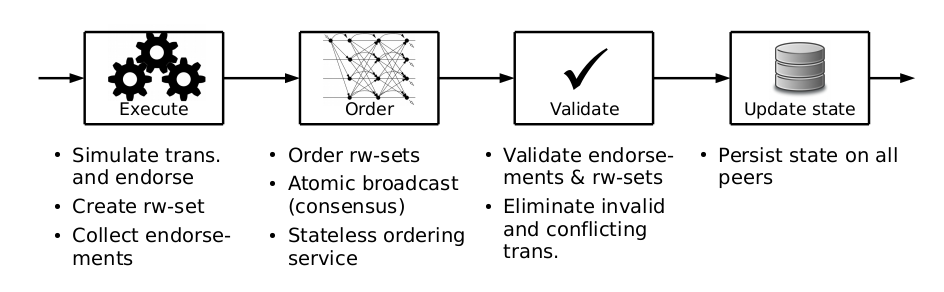
\includegraphics[width=1\linewidth]{imgs/executeOrderValidate.png}
  \caption{\label{fig:executeorder} Execute-order-validate architecture of
  Fabric (Source: IBM, 2018)}
\end{figure}

Fabric introduces the execute-order-validate Blockchain architecture as shown
on Figure~\ref{fig:executeorder} and does not follow the standard order-execute
design illustrated on Figure~\ref{fig:orderexecute} \cite{Androulaki2018}. In
this architecture, when a client sends transactions to the peers specified by
endorsement policy. Each transaction is then executed and its output is
recorded. After execution, transactions enter the ordering phase. An ordered
sequence of transactions grouped into blocks are produced using the consensus
mechanism. Then, these blocks are broadcast to all peers. Fabric orders the
transaction outputs computed during the execution phase. Each peer then
validates state changes according to the endorsement policy and the consistency
of the execution in the validation phase. All peers validate the transactions
in the same order and validation is deterministic. In this sense, Fabric
introduces a novel hybrid replication paradigm in the Byzantine
model~\cite{Androulaki2018}. This model combines passive replication, which is
the pre-consensus computation of state updates, with active replication, the
post-consensus validation of execution results and state changes.

\begin{figure}[h]
  \centering
  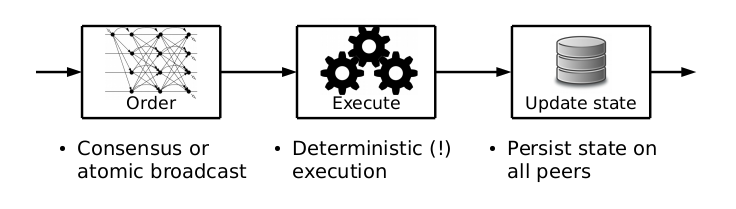
\includegraphics[width=0.8\linewidth]{imgs/orderExecuteArchitecture.png}
  \caption{\label{fig:orderexecute} Order-execute architecture in Replicated
  Services Like Ethereum (Source: IBM, 2018)}
\end{figure}

On the other hand, the order-execute architecture is conceptually simple,
leading it to be currently widely implemented in replicated services such as
Blockchain. In this architecture the transactions are executed sequentially on
all peers which limits the maximum number of simultaneous transactions that can
be achieved.  Additionally a Denial of Service (\textbf{DOS}) attack can be
mounted just by deploying a slow performing smart contract or one with an
infinite loop to the network since the Blockchain forms a distributed computing
engine.  To cope with this issue, public programmable Blockchains with an
associated cryptocurrency, account for the execution cost of executing of the
program.

In Fabric all nodes that participate in the network have an identity, as
provided by a modular Membership Service Provider (\textbf{MSP}).  A
\textbf{MSP} is a component that aims to offer the abstraction of a membership
operation architecture meaning that all identities are only allowed to
participate if verified to be considered trustworthy.  The \textbf{MSP}
maintains the identities of all nodes in the system and is responsible for
issuing credentials that are used for node authentication and authorization. An
\textbf{MSP} may define their own notion of identity, and the rules by which
those identities are governed and authenticated using signature generation and
verification~\cite{HyperledgerFabricDocs2017}.

Fabric also assigns different roles to peers. Nodes in Fabric network can have
one or more, of these three roles:

\begin{itemize}
  \item Clients submit transaction proposals for execution, help orchestrate
    the execution phase, and broadcast transactions for ordering.

  \item Peers execute transaction proposals and validate transactions.  All
    peers maintain the ledger, where all transactions  are recorded in the form
    of a hash chain, as well as the state, a succinct representation of the
    latest ledger state. Not all peers execute all transactions.

  \item Ordering Service Nodes (\textbf{OSN}) or orderers are the nodes that
    collectively form the ordering service. In short, the ordering service
    establishes the total order of all transactions in Fabric, where each
    transaction contains state updates and dependencies computed during the
    execution phase, along with cryptographic signatures of the endorsing peers
    defined in the endorsing policy of the transaction. Orderers are entirely
    unaware of the application state, and do not participate in the execution
    nor in the validation of transactions. This design choice renders consensus
    in Fabric as modular as possible and simplifies the replacement of
    consensus protocols in Fabric. 
\end{itemize}

Looking ahead, Hyperledger Fabric will continue to focus on privacy and
confidentiality with v1.2 being recently released, v1.3 and 1.4 expected to be
out this year with further emphasis on these aspects in a regular quarterly
cadence~\cite{hyperledgerRoadmap2018}.
